\documentclass{article}
\usepackage{amsmath}
\usepackage{tikz}

\begin{document}

The $\frac{\mathbb{R} \times [-1,1]}{\mathbb{Z}_2}$ geometry realizing the 4d lift of $B_c$ has an orbifold singularity. It can be smoothed out to the shape on the right-hand side of the picture, with the orbifold singularity mapped to an interior point. We pick the initial corner so that no co-dimension 2 defect is present at the interior point.

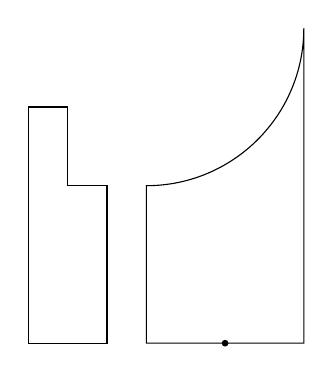
\begin{tikzpicture}[scale=0.5]
    % Left panel - Original Shape
    \draw (0,0) -- (0,6) -- (1,6) -- (1,4) -- (2,4) -- (2,0) -- cycle;
    
    % Right panel - Smoothed Shape
    \draw (7,0) -- (7,8) arc (0:-90:4) -- (3,0) -- cycle;
    \filldraw[black] (5,0) circle (2pt);
\end{tikzpicture}

\end{document}